\documentclass[10pt]{article}
\usepackage[polish]{babel}
\usepackage[utf8]{inputenc}
\usepackage[T1]{fontenc}
\usepackage{amsmath}
\usepackage{amsfonts}
\usepackage{amssymb}
\usepackage[version=4]{mhchem}
\usepackage{stmaryrd}
\usepackage{graphicx}
\usepackage[export]{adjustbox}
\graphicspath{ {./images/} }

\title{KLASY PO SZKOLE PODSTAWOWEJ }

\author{}
\date{}


\begin{document}
\maketitle
\begin{enumerate}
  \item Sprawdź, czy liczby naturalne od 1 do 18 można umieścić w wierzchołkach i na środkach krawędzi ośmiościanu foremnego tak, aby każda liczba leżąca na krawędzi ośmiościanu była średnią arytmetyczną liczb leżących na jej końcach. Jeśli można, pokaż, jak to zrobić, jeśli nie można, uzasadnij, dlaczego.
  \item Znajdź liczby naturalne \(a, b, n\), spełniające równość:
\end{enumerate}

\[
\frac{1}{a}+\frac{1}{b}=n
\]

\begin{enumerate}
  \setcounter{enumi}{2}
  \item W trójkącie \(A B C\) punkt \(I\) jest środkiem okręgu wpisanego. Na boku \(A B\) obieramy takie punkty \(P\) i \(Q\), że \(I P \| A C\) oraz \(I Q \| B C\). Udowodnij, że obwód trójkąta \(P I Q\) ma taką samą długość jak bok \(A B\).\\
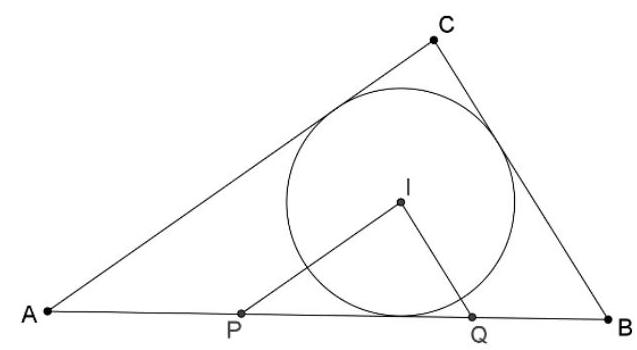
\includegraphics[max width=\textwidth, center]{2024_11_21_7df58923022be014b7d0g-1(1)}
\end{enumerate}

\section*{KLASY PO GIMNAZJUM}
\begin{enumerate}
  \item Dany jest kwadrat \(A B C D\). Na bokach BC i CD wybrano odpowiednio punkty E i F tak, że kąt EAF ma \(45^{\circ}\). Udowodnij, że pole trójkąta AEF jest równe sumie pól trójkątów ABE i AFD.
  \item W konfiguracji z zadania 1 punkty H oraz I są odpowiednio punktami wspólnymi przekątnej BD z odcinkami AE i AF. Udowodnij, że \(|\mathrm{IH}|^{2}=|\mathrm{DI}|^{2}+|\mathrm{HB}|^{2}\)
  \item W konfiguracji z zadania 1 punkt O jest środkiem okręgu opisanego na trójkącie AEF, a punkt W środkiem okręgu wpisanego w trójkąt EFC. Udowodnij, że punkt O jest środkiem odcinka AW.\\
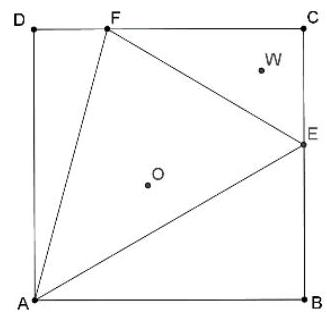
\includegraphics[max width=\textwidth, center]{2024_11_21_7df58923022be014b7d0g-1}
\end{enumerate}

\end{document}